\subsection{Ontology in Blockchain}
\label{subsec:ontology-in-blockchain}

Konsep ontology di dalam blockchain adalah sebuah pendekatan yang berupaya untuk memetakan fitur dan konsep dari blockchain secara formal dan \textit{shared} untuk mendukung \textit{interoperability} \parencite{9770809} dan mewujudkan visi \textit{semantic} blockchain \parencite{hector2020blondie}.

\subsubsection{EthOn}
\label{subsubsec:ethon}

\begin{figure}[ht]
	\centering
	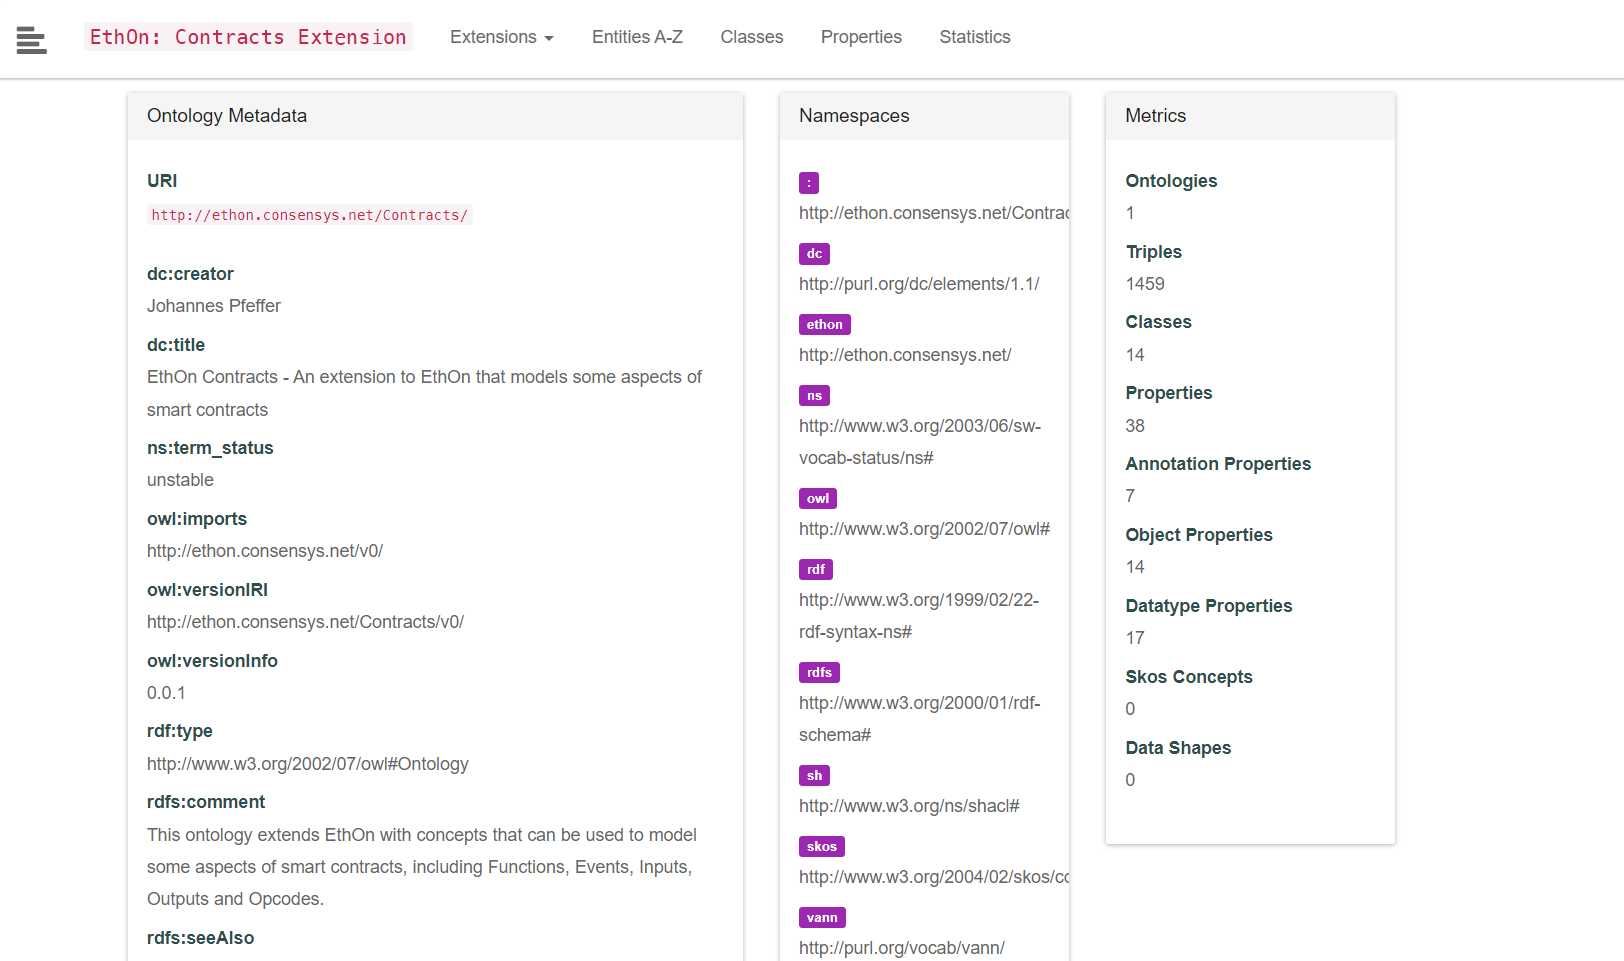
\includegraphics[width=0.7\textwidth]{resources/chapter-2/ethon.png}
	\caption{Visualisasi EthOn \parencite{ethon2024}}
	\label{image:ethon}
\end{figure}

EthOn adalah sebuah ontology yang dirancang secara spesifik untuk ekosistem Ethereum untuk merepresentasikan struktur, komponen, dan relasi di dalam Blockchain Ethereum. Visualisasi EthOn dapat dilihat pada gambar \ref{image:ethon}. EthOn menyediakan \textit{semantic framework} untuk standarisasi dan interpretasi data kompleks yang terasosiasi dengan transaksi, Smart Contracts, blok, akun, dan entitas lainnya. Ontology ini memberikan cara untuk menginterpretasikan data dengan cara yang lebih terstruktur dan berarti, mendukung \textit{interoperability}, dan integrasi data \parencite{pfeffer2016ethon}.

\subsubsection{BLONDiE}
\label{subsubsec:blondie}

\begin{figure}[ht]
	\centering
	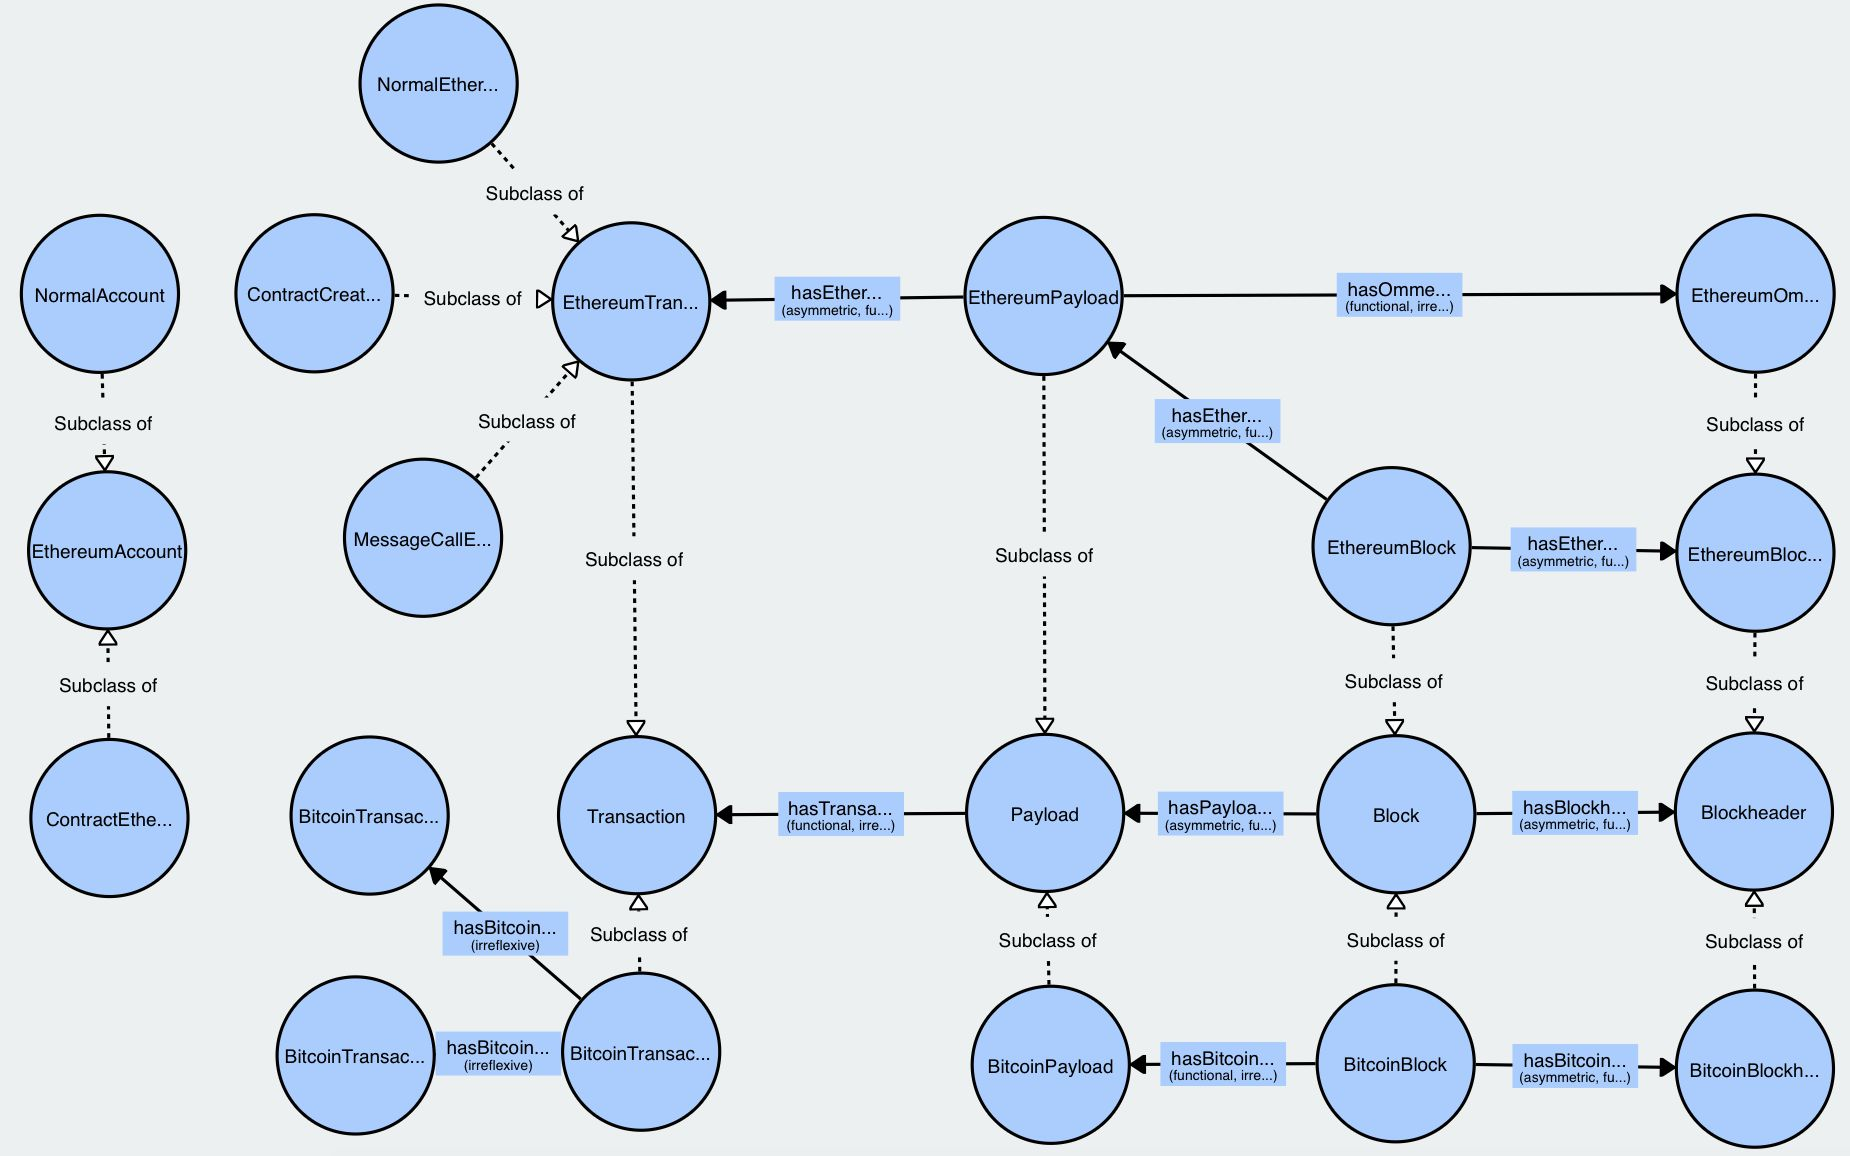
\includegraphics[width=1\textwidth]{resources/chapter-2/blondie-visualization.jpg}
	\caption{Visualisasi Ontology BLONDiE \parencite{third2017linked}}
	\label{image:blondie-visualization}
\end{figure}

BLONDiE adalah singkatan dari blockchain Ontology with Dynamic Extensibility, yang merupakan sebuah \textit{vocabulary} untuk merepresentasikan konsep di dalam blockchain dengan potensi untuk ekstensi. Ontology ini terdiri atas 23 \textit{class}, 11 \textit{object properties}, dan 64 \textit{data properties} \parencite{hector2020blondie}. Gambar \ref{image:blondie-visualization} memvisualisasikan ontology BLONDiE.